\section{GlueX DIRC Detector Design}

This chapter will describe the purpose and general design of the \gluex DIRC.
\vspace{0.5cm}

The \gluex DIRC detector~\cite{dirc} is designed to improve the particle identification (PID) capabilities in the forward region of the \gluex~\cite{gluex1, gluex2} detector, located in Hall D at the Jefferson Lab. The baseline PID in the forward region of the \gluex detector is done by a Time-Of-Flight (TOF) wall, which separates kaons from pions up to momentum of about 2 \gev/c. The \gluex DIRC is designed to provide clean separation between kaons and pions with at least three standard deviations for momenta up to 4 \gev/c.

\begin{figure}[!htb]
\centering
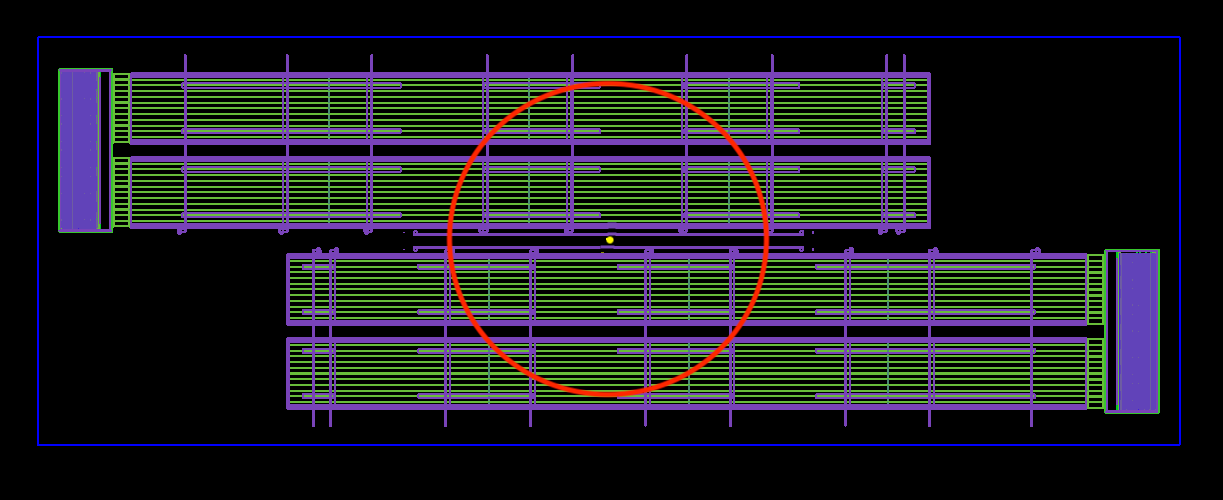
\includegraphics[width=0.9\textwidth]{pics/sim1.png}
\caption{\label{pic:sim}
The downstream view of the \gluex DIRC optical system (from the simulation). The beam going into the page is shown in yellow. The red circle shows the polar angle acceptance ($11^{\circ}$ degrees).
The blue box around the detector is the auxiliary volume \texttt{DIRC} containing all the DIRC components, which can be activated/deactivated in the Hall D geometry to insert/remove the \gluex DIRC to/from the \gluex detector simulation.}
\end{figure}

The \gluex DIRC forms a wall about 5 m away from the target directly upstream of the TOF detector. The DIRC consists of four \babar DIRC~\cite{bdirc1} bar boxes and covers the polar angle range from 2\mydeg to 11\mydeg (see Fig.~\ref{pic:sim}). Two bar boxes located above the beam line are attached to a photon camera\footnote{For historical reasons, there are two terms: ``photon camera'' and ``optical box''. Essentially, they mean the same in the current document and can be used interchangeably.} located to the left of the beam. Another pair of bar boxes, covering the acceptance below the beam line, is attached to the second photon camera, located to the right of the beam. The support structure of the DIRC (shown in Fig.~\ref{pic:support}) allows the pairs of bar boxes to be moved out of the active area of the detector for experiments requiring minimal material budget in front of the forward calorimeter.

The \babar DIRC bar boxes number 0, 1, 10, 11 (out of twelve) were selected for the \gluex DIRC. They were brought to Hall D by truck from SLAC, where all the bar boxes had been stored after the \babar experiment was disassembled in 2010. The bar box, shown in Fig.~\ref{pic:bbox}, contains $12$ long radiator bars ($35 \times 17.25 \times 4900 $ mm$^3$) inside. A small wedge is attached to the readout end of each bar. Bar boxes are to be used without modifications, which means that the small wedges have to stay in the optical system of the \gluex DIRC.

\begin{figure}[h]
\centering
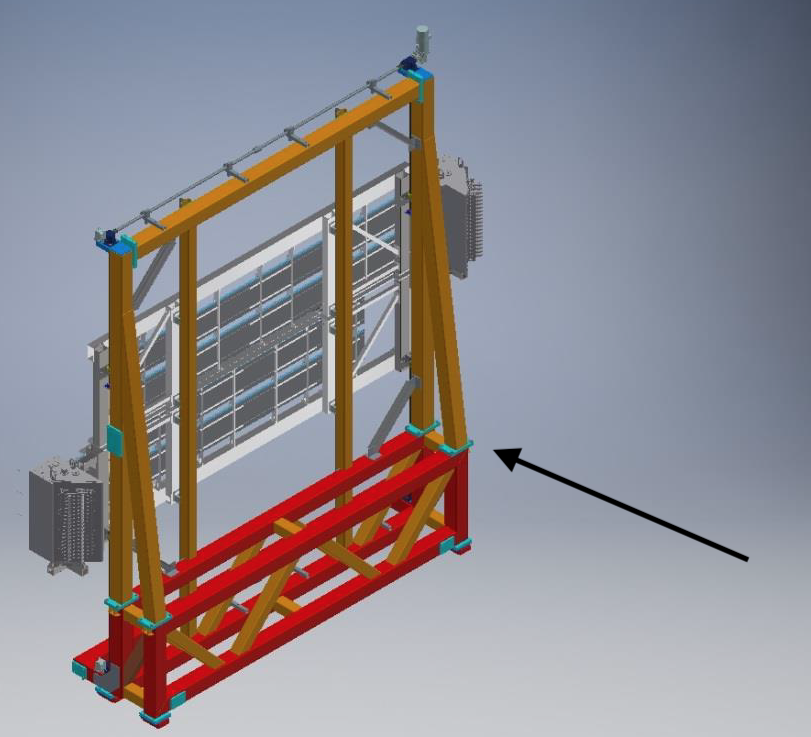
\includegraphics[width=0.37\textwidth]{pics/support.png} \hspace{0.2cm}
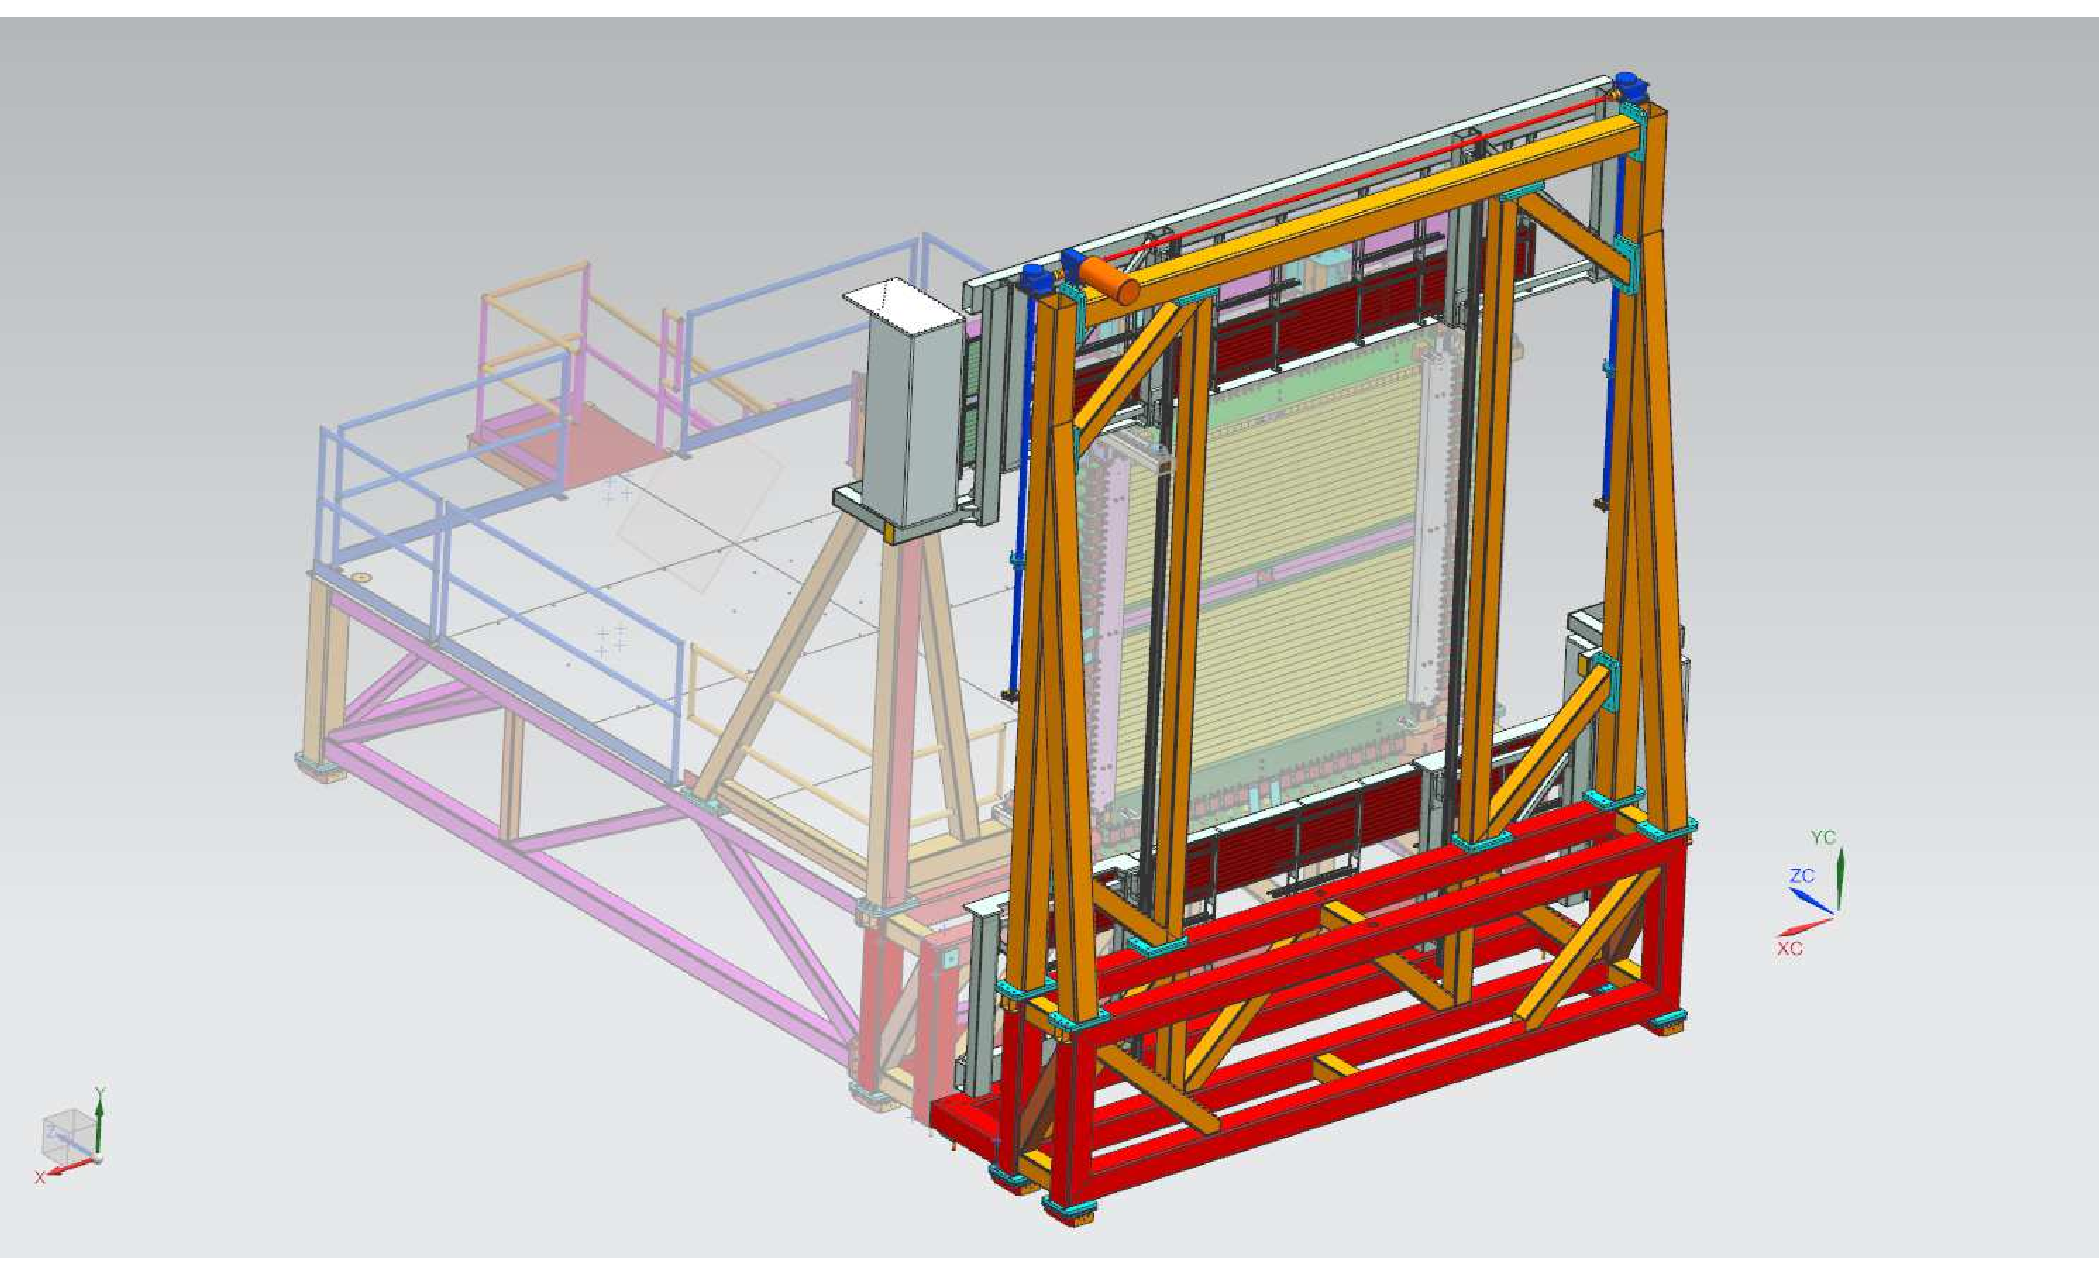
\includegraphics[width=0.56\textwidth]{pics/Full_Assy_Iso-retracted.pdf}
\caption{\label{pic:support}} A technical drawing of the support structure with the DIRC optical system installed. 
The bar boxes slide up and down within the orange frame: the DIRC is in working position (left) and retracted (right). 
The beam is coming from the right.
\end{figure}

\begin{figure}[!h]
\centering
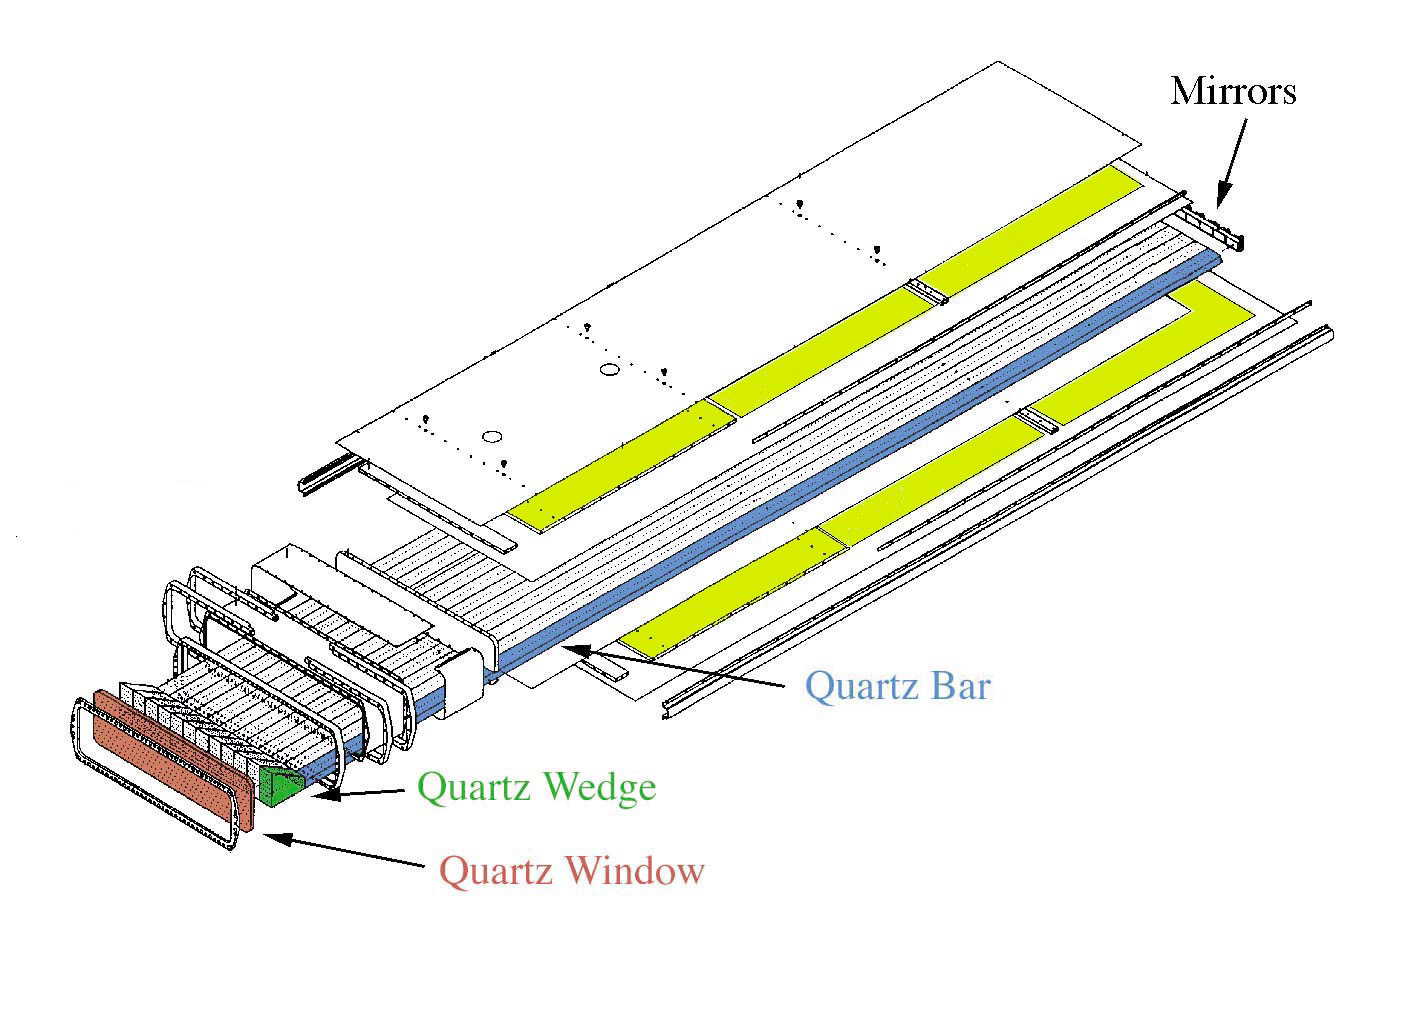
\includegraphics[width=0.8\textwidth]{pics/bab_col.jpg}
\caption{\label{pic:bbox} Schematic of the \babar DIRC bar box assembly~\cite{bdirc1}. The single radiator bar is highlighted in blue, the small wedge in green.}
\end{figure}

\begin{figure}[!h]
%\begin{center}
\begin{minipage}{0.6\textwidth}
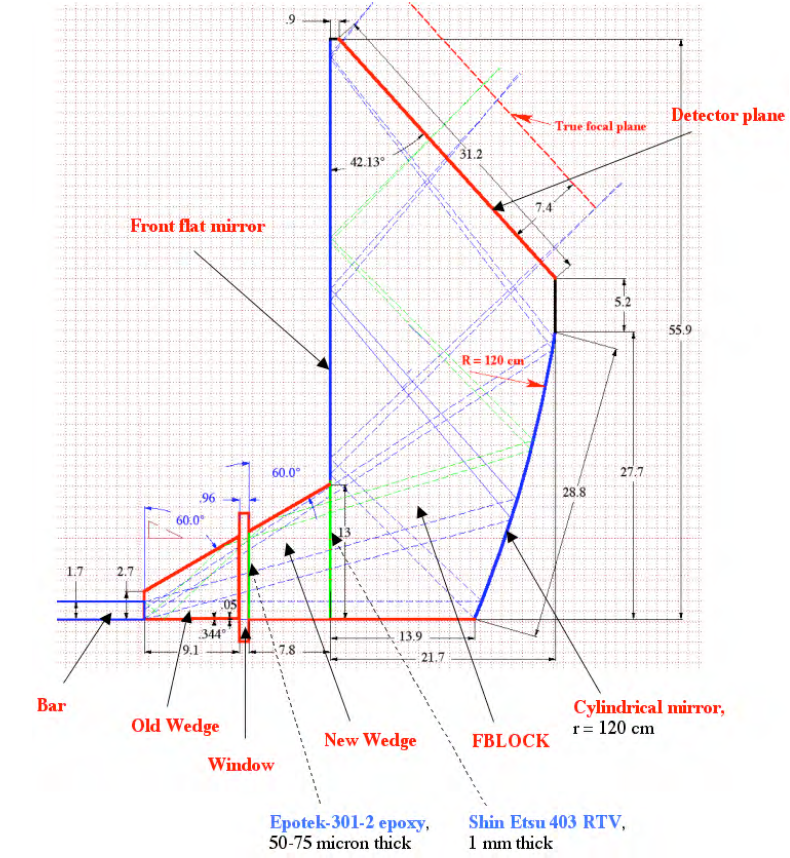
\includegraphics[width=0.9\textwidth]{pics/fdirc.png} 
\end{minipage} 
\begin{minipage}{0.4\textwidth}
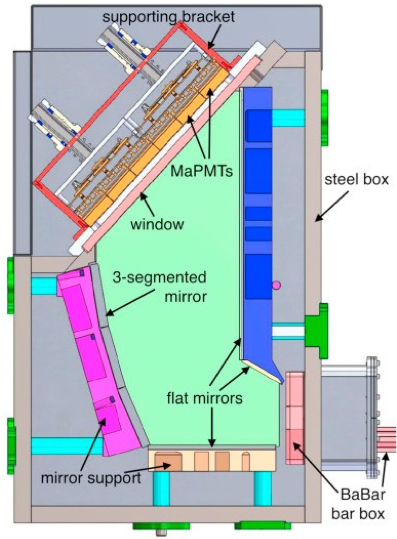
\includegraphics[width=0.9\textwidth]{pics/pc.png}\\
\vspace{0.5cm}
\end{minipage}
%\end{center}
\caption{\label{pic:ob} Shape of the photon camera for the SuperB~\cite{fdirc} (left) and for the \gluex DIRC~\cite{tdr} (right). The photon camera for the \gluex DIRC is a steel tank filled with distilled water with immersed mirrors to approximate the shape of the photon camera for the SuperB FDIRC.}
\end{figure}

The design of the photon camera is based on the SuperB FDIRC\footnote{FDIRC was designed to be the successor of the \babar DIRC, but the the SuperB project was cancelled in 2012.} prototype~\cite{fdirc} developed at SLAC. Figure~\ref{pic:ob} shows both cameras. The FDIRC photon camera design was based on compact focussing blocks made of fused silica, one for each bar box in a barrel. For the \gluex DIRC planar orientation one common camera, filled with distilled water, are used for two bar boxes together. This design with wider cameras (the width is $983$ mm) reduces the fraction of photons reflecting off the sides, simplifying the hit pattern and removing ambiguities in the reconstruction (reconstruction details see in Sec.~\ref{sec:gr} and Sec.~\ref{sec:ti}). Another important modification of the photon camera is the approximation of the cylindrical mirror by a set of three flat segments for simplicity in alignment and construction. 

The \gluex DIRC is read out by an array of Hamamatsu H12700 Multi-Anode PMTs (MaPMTs). Each photon camera is read out by an array of $5 \times 18$ MaPMTs. One edge row of $18$ MaPMTs on each camera is substituted by dummies. This allows to use fewer PMTs. Simulation studies showed that there is no performance loss due to removing one row of PMTs. The photosensors are coupled to the window of the optical box using custom-made silicone pads to minimise the photon loss between the window of the photon camera and MaPMTs. 

The electronics boards are the same as for the CLAS12 RICH in Hall B. They are compatible with the generic JLab DAQ systems.
